\subsection{Standard Model W+Jets}
\label{sec:Bkg:wjet}

\indent A $W$ boson produced in conjunction with QCD jets ($W$+jets) consists our largest sub-dominant background.  $W$+jets makes up 5 percent of the total background in the SR.  However the distribution of $W$+jets is not uniform across $\RISR$.  $W$+jets can reach around 15 percent of all background in the SR bins with the largest $\RISR$.  This means the $W$+jets contribution mostly affects high stop mass samples because those signal samples peak at high $\RISR$. \\

\indent We estimate $W$+Jets using an one lepton control region defined in table \ref{tab:WJetCR}..  The one lepton $W$+jet CR is designed to ensure high $W$+jet purity.   All one lepton CRs are mutually exclusive including the ttbar, $W$+jets and single top CR. \\

\begin{table}[htpb]
  \begin{center}
    \begin{tabular}{c|c}
      \hline \hline
                                      & CRW                \\ \hline
      Number of leptons             & 1                                          \\ \hline
      Number of jets (incl. lepton) & $\geq 4$                                     \\ \hline
      $\pt$ of jets (incl. lepton)  & (80,80,40,40) GeV                            \\ \hline
      \mindphijettwomet             & $> 0.4$                                      \\ \hline
      $\met$                        & $>250$ GeV                                   \\ \hline
      \mtlepmet                     & ($>30, <100$ GeV) \\ \hline
      Number of $b$-jets            & $=1$                            \\ \hline
      \mantikttwelvezero            & $<60\,$GeV         \\ \hline
      \mindrblep                    & $>2.0$             \\ \hline \hline
    \end{tabular}
  \end{center}
  \caption{Summary of the selection for the one lepton $W$+jets control region.}
  \label{tab:WJetCR}
\end{table}

\indent The {\tt Signal} lepton is treated as a jet for the jet multiplicity and the jet $\pt$ requirements.  The mass requirement on the large R jet $\mantikttwelvezero < 60 \gev$ rejects events with reconstructed boosted tops.  The $\mtlepmet$ selection ensures that the transverse mass is consistent with those originating from a $W$ boson.  \\

\indent Orthogonality between the $W$+jet CR and the single top CR is ensured by the requirement on the number of $b$-jets.  Orthogonality between ttbar CR and $W$+jet CR is ensured by the selection on $\Delta R(b_{0,1},\ell)_{\mathrm{min}}$, defined as the minimum $\Delta R$ between the two jets with the highest b-tag value and the selected lepton.  \\

\indent  Distributions of select kinematic variables in the $\Wjets$ control region are shown in figure ~\ref{fig:CRWpts}.  The MC background has been normalized to data by performing a simultaneous fit to all CRs.  The hashed bands on the total SM background correspond to the total experimental systematical uncertainty plus the MC statistical uncertainty.  The yield in the $\Wjets$ CR is given in table~\ref{tab:CRW_yields}.  \\

\indent  Data and MC are compatible to within statistical uncertainty.  No strong trends are observed in the data to MC ratios in any of the distributions. \\

\begin{table}[!htb]
  \centering
  \begin{tabular}{c|c}
\hline\hline
\multicolumn{2}{c}{\bf CRW (60\% purity)} \\ \hline 
Z & 1.99 $\pm$ 0.45 \\
dibosons & 9.85 $\pm$ 1.76 \\
ttbar & 128.42 $\pm$ 3.82 \\
singleTop & 51.14 $\pm$ 3.37 \\
ttV & 1.07 $\pm$ 0.16 \\
W & 288.12 $\pm$ 8.86 \\
\hline
Total MC & 480.58 $\pm$ 10.38 \\
Data & 531.00 $\pm$ 23.04 \\
 \hline
SF & 1.17 $\pm$ 0.10 \\
\hline\hline
\end{tabular}

  \caption{Yields in the $\Wjets$ CR with \intlumi\ \ifb\ of data.  }
  \label{tab:CRW_yields}
\end{table}

\begin{figure}[!htb]
  \centering
  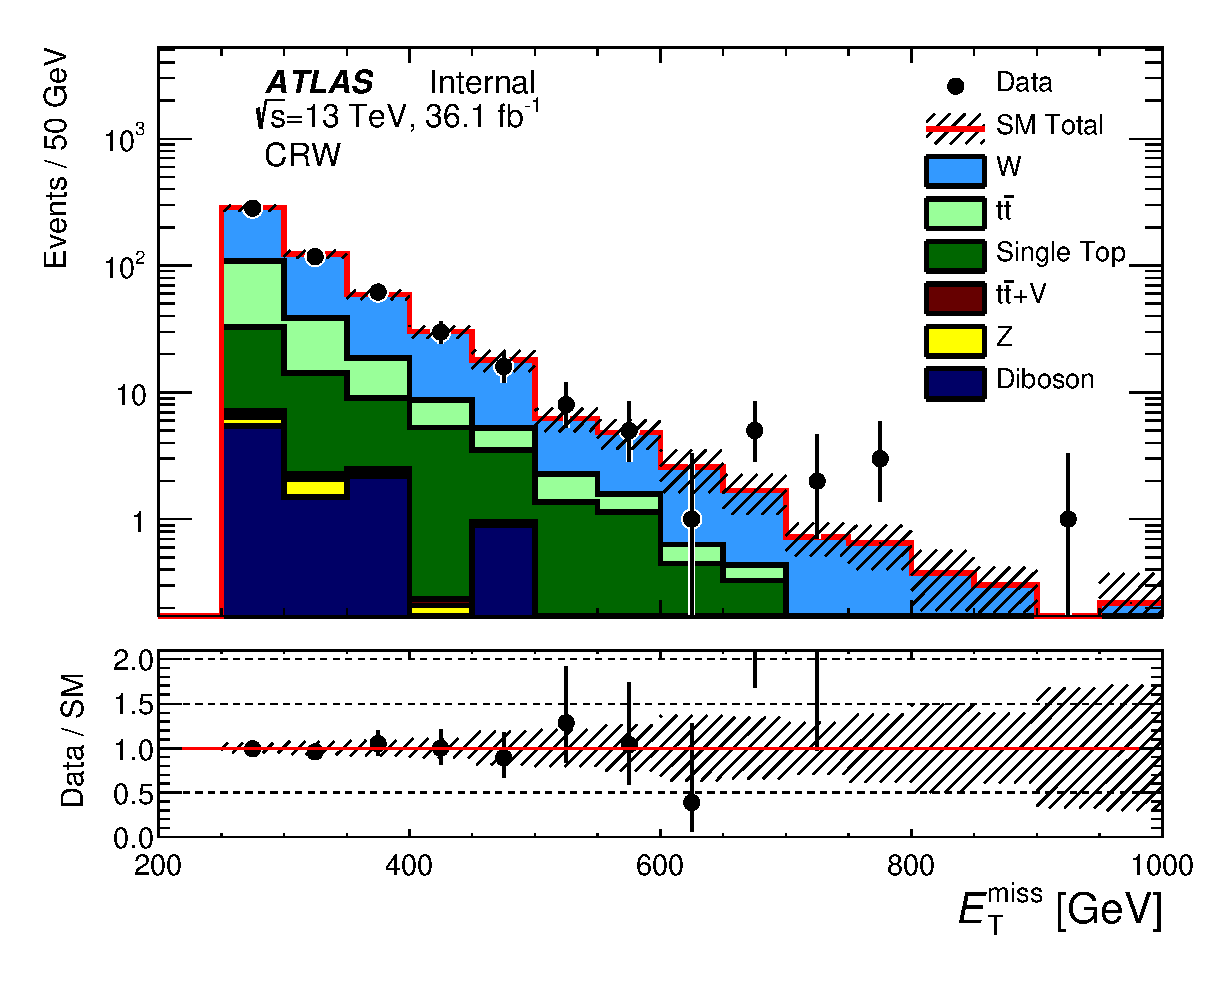
\includegraphics[width=0.45\textwidth]{figures/wJets/postfit/Met_CRW_log.eps}
    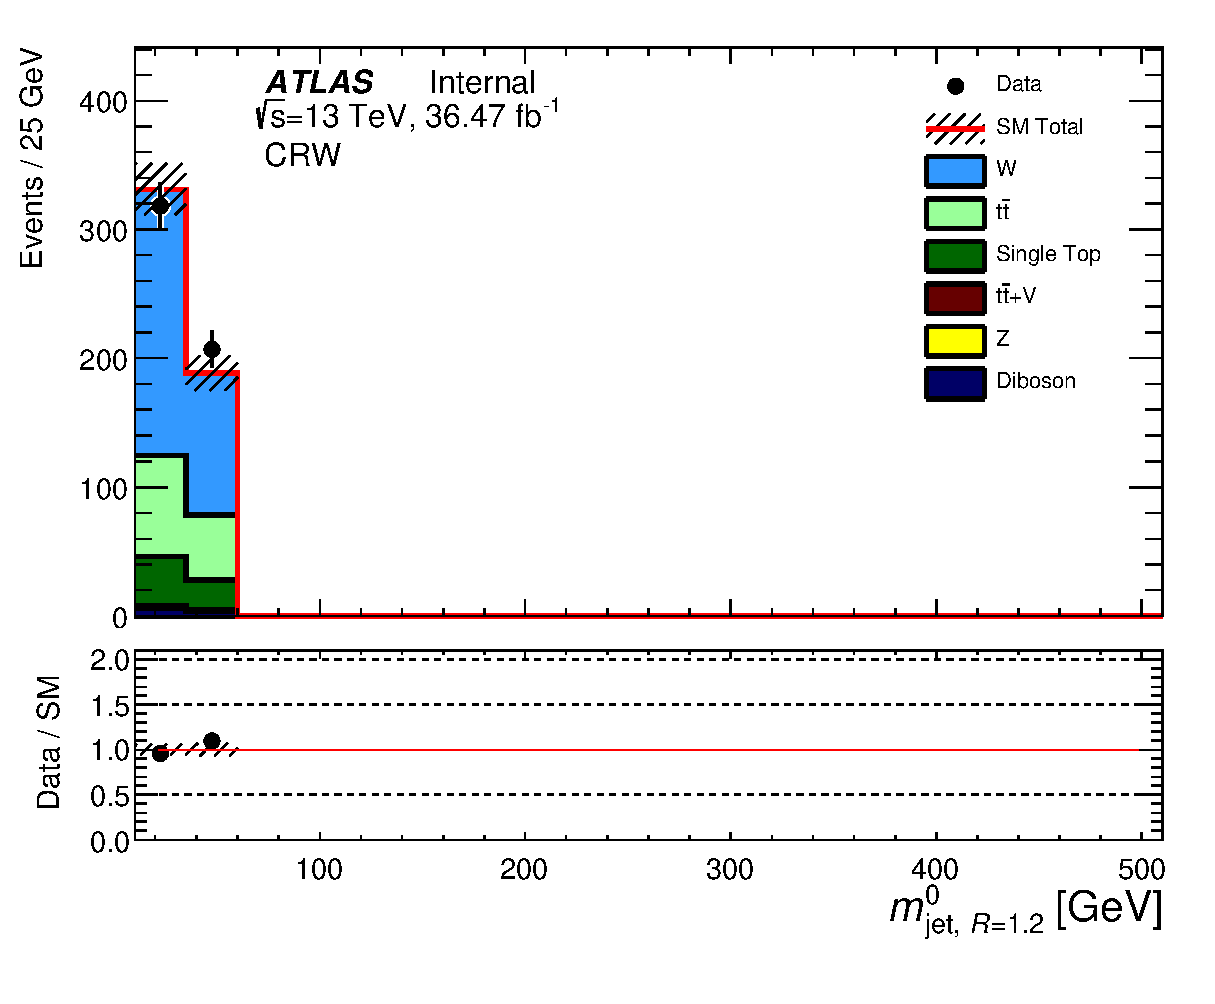
\includegraphics[width=0.45\textwidth]{figures/wJets/postfit/AntiKt12M_0__CRW.eps}
  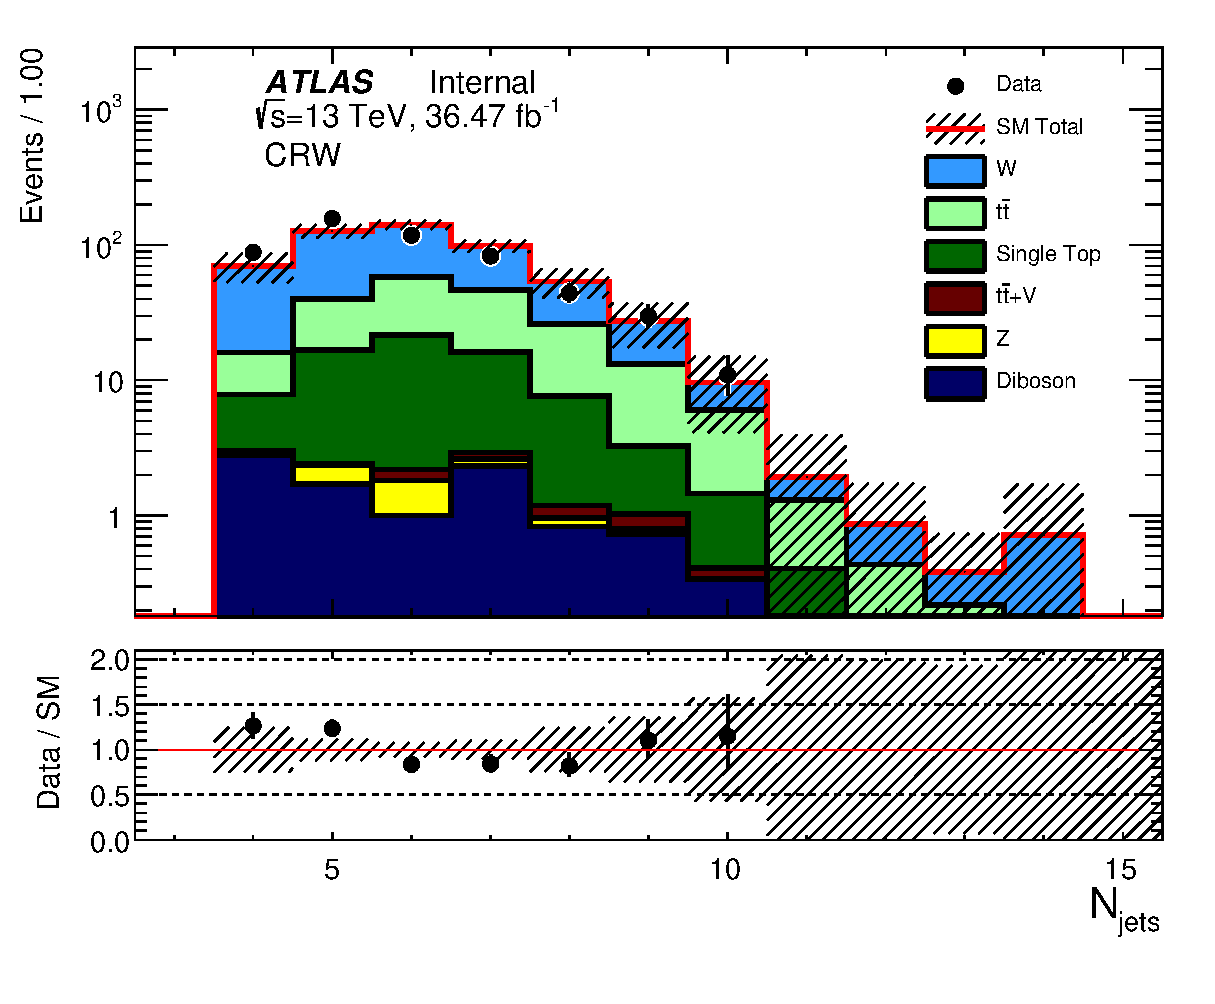
\includegraphics[width=0.45\textwidth]{figures/wJets/postfit/NJets_CRW_log.eps}
  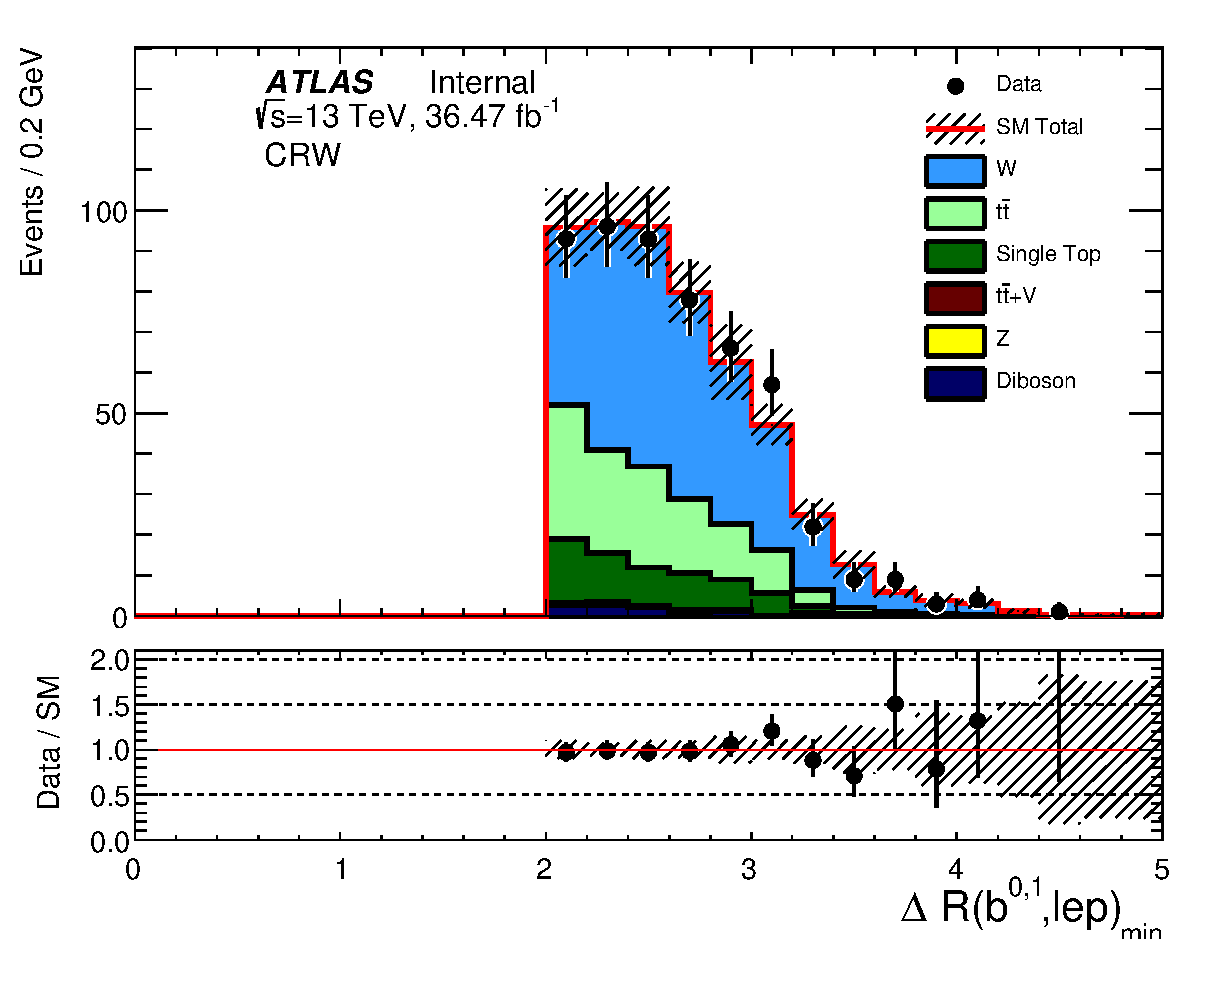
\includegraphics[width=0.45\textwidth]{figures/wJets/postfit/MinDRBLep_CRW.eps}]
  \caption{Postfit data/MC comparisons in the $\Wjets$ CR. From left to right and top to bottom, the variables shown are $\met$, $\mtlepmet$, $\mantikttwelvezero$ and $\mindrblep$. The expected SM background has been normalized to data in the CR by performing a simultaneous fit to all background CR.  The hatched band on the total SM background correspond to the total experimental systematic uncertainty plus the MC statistical uncertainty.}
  \label{fig:CRWpts}
\end{figure}


